\documentclass[12pt]{exam}


\usepackage{cmap, type1ec}
\usepackage[T2A]{fontenc}
\usepackage[utf8]{inputenc}
\usepackage[russian]{babel}

\usepackage{xcolor}
\usepackage{hyperref}
\usepackage{alltt}

\hypersetup{%
  colorlinks=false,% hyperlinks will be black
  linkbordercolor=blue,% hyperlink borders will be red
  pdfborderstyle={/S/U/W 1}% border style will be underline of width 1pt
}

\usepackage[margin=1in]{geometry}
\usepackage{amsmath,amssymb}
\usepackage{multicol}
\usepackage{etoolbox}

\usepackage{float}
\usepackage{siunitx}

\usepackage{tikz}
\usetikzlibrary{trees}
\usetikzlibrary{shapes.geometric}
\usetikzlibrary{positioning}

\newcommand{\class}{Теория алгоритмов}
\newcommand{\term}{Весенний семестр 2017}
\newcommand{\examnum}{Пересдача}
\newcommand{\examdate}{25 сентября 2017}
\newcommand{\timelimit}{18:10 -- 20:10}

\pagestyle{head}
\firstpageheader{}{}{}
\runningheader{\class}{\examnum\ - Страница \thepage\ из \numpages}{\examdate}
\runningheadrule

\providecommand{\abs}[1]{\left\lvert{#1}\right\rvert}

\renewcommand{\solutiontitle}{}

\makeatletter
\newcommand{\iftoggleverb}[1]{%
  \ifcsdef{etb@tgl@#1}
    {\csname etb@tgl@#1\endcsname\iftrue\iffalse}
    {\etb@noglobal\etb@err@notoggle{#1}\iffalse}%
}
\makeatother

\graphicspath{{./figures/}}

\begin{document}

\noindent
\begin{tabular*}{\textwidth}{l @{\extracolsep{\fill}} r @{\extracolsep{6pt}} l}
\textbf{\class} & \textbf{Студент:} & \makebox[3in]{\hrulefill}\\
\textbf{\term} &&\\
\textbf{\examnum} &&\\
\textbf{\examdate} \\
\textbf{\timelimit}
\end{tabular*}\\
\rule[2ex]{\textwidth}{2pt}%
% \begin{center}
% Оценки (заполняется проверяющими)\\
% \addpoints
% \gradetable[v][questions]
% \end{center}
% \noindent
% \rule[2ex]{\textwidth}{2pt}

\begin{questions}

\question[1] Что из этого не входит в $O(n^2)$?
\begin{checkboxes}
\choice $(15^{10}) * n + 12099$
\choice $n^{1.98}$
\CorrectChoice $n^3 / \sqrt{n}$
\choice $(2^{20}) * n$
\end{checkboxes}

\question[3] На диске имеется файл с 1 миллионом чисел. RAM компьютера не хватает, чтобы загрузить все числа в память. В таких условиях, с помощью какой структуры данных получится наиболее эффективно найти 10 {\em наибольших} чисел?
\begin{checkboxes}
\CorrectChoice Min heap
\choice Max heap
\choice Бинарное дерево поиска
\choice Отсортированный массив
\end{checkboxes}

\question[1] Какую из операций нельзя выполнить за $O(1)$ в отсортированном массиве, в котором все элементы различны?
\begin{checkboxes}
\choice Найти $i$-й наибольший элемент
\CorrectChoice Удалить элемент
\choice Найти $i$-й наименьший элемент
\choice Всё перечисленное
\end{checkboxes}

\question[1] Что из перечисленного верно для стека, реализованного через связный список?
\begin{checkboxes}
\choice Если {\tt push} добавляет элементы в начало списка, то {\tt pop} удаляет их с конца списка
\choice Если {\tt push} добавляет элементы в конец списка, то {\tt pop} удаляет их из начала списка
\choice Всё вышеперечисленное
\CorrectChoice Ничего из вышеперечисленного
\end{checkboxes}


\question[2] Дана пустая хэш-таблица размера 10, использующая открытую адресацию со стратегией linear probing. Используется хэш-функция $h(k) = k \mod 10$. После вставки шести элементов хэш-таблица выглядит так:
\begin{figure}[H]
  \begin{center}
    \begin{tabular}{|c|c|c|c|c|c|c|c|c|c|}
    \hline
    0 & 1 & 2  & 3  & 4  & 5  & 6  & 7  & 8 & 9 \\ \hline
    ~ & ~ & 42 & 23 & 34 & 52 & 46 & 33 & ~ & ~ \\ \hline
    \end{tabular}
  \end{center}
\end{figure}
В каком порядке могли быть вставлены эти элементы?

\begin{checkboxes}
\choice {\tt 46, 42, 34, 52, 23, 33}
\choice {\tt 34, 42, 23, 52, 33, 46}
\CorrectChoice {\tt 46, 34, 42, 23, 52, 33}
\choice {\tt 42, 46, 33, 23, 34, 52}
\end{checkboxes}

\question[1] Что из перечисленного {\em не является} in-place алгоритмом?
\begin{checkboxes}
\choice Insertion sort
\choice Selection sort
\CorrectChoice Merge sort
\choice Heap sort
\end{checkboxes}

\question[1] Какой из алгоритмов сортировки исполняется наименьшее время на почти отсортированных массивах, где всего 1-2 элемента стоят не на своих местах? 
\begin{checkboxes}
\choice Quick Sort
\choice Heap Sort
\choice Merge Sort
\CorrectChoice Insertion Sort
\end{checkboxes}

\question[1] При сортировке массива из восьми чисел алгоритмом Quicksort после первой процедуры partition массивы выглядит так:
$$
2~~5~~1~~7~~9~~12~~11~~10
$$
Отметьте корректное утверждение:
\begin{checkboxes}
\CorrectChoice Опорный элемент может быть либо 7, либо 9
\choice Опорный элемент может быть 7, но точно не 9
\choice Опорный элемент может быть 9, но точно не 7
\choice Ни 7, ни 9 не являются опорными элементами
\end{checkboxes}

\question[1] Сколько различных бинарных деревьев можно построить из трёх немаркированых узлов?
\begin{checkboxes}
\choice 1
\CorrectChoice 5
\choice 4
\choice 3
\end{checkboxes}

\question[1] В пустое [не самобалансирующееся] бинарное дерево поиска добавляются числа в следующем порядке:
$$
10~~1~~3~~5~~15~~12~~16
$$
Какова получившаяся высота дерева (максимальное количество рёбер от корня до листьев)?
\begin{checkboxes}
\choice 2
\CorrectChoice 3
\choice 4
\choice 6
\end{checkboxes}

\question[1] Что из перечисленного является общим во всех типах обходов двоичного дерева (inorder, preorder, postorder)?
\begin{checkboxes}
\choice Корень посещается перед правым поддеревом
\CorrectChoice Левое поддерево всегда посещается перед правым поддеревом
\choice Корень посещается после левого поддерева
\choice Всё вышеперечисленное
\choice Ничего из вышеперечисленного
\end{checkboxes}

\question[1] Какой алгоритм позволяет наиболее эффективно определить наличие цикла в графе?
\begin{checkboxes}
\CorrectChoice Поиск в глубину (DFS)
\choice Поиск в ширину (BFS)
\choice Алгоритм Прима для MST
\choice Алгоритм Краскала для MST
\end{checkboxes}

\question[1] Чему равна сумма всех степеней вершин неориентированного графа $G=(V,E)$?
\begin{checkboxes}
\choice $\abs{E}$
\CorrectChoice $2\abs{E}$
\choice $\abs{V}$
\choice $2\abs{V}$
\end{checkboxes}

\question[2] Пусть реализован поиск в ширину, где для хранения соседних вершин используется очередь. Обходим граф:
\begin{figure}[H]
  \begin{center}
    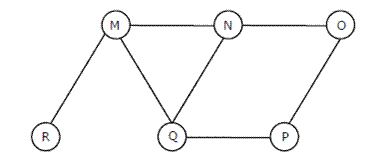
\includegraphics[width=10cm]{bfs.png}
  \end{center}
\end{figure}
Какой из перечисленных путей возможен при таком обходе?
\begin{checkboxes}
\choice MNOPQR
\choice NQMPOR
\CorrectChoice QMNPRO
\choice QMNPOR
\end{checkboxes}

\question[2] Используя алгоритм Дейкстры, ищем кратчайшие пути в данном графе с источником в вершине P:
\begin{figure}[H]
  \begin{center}
    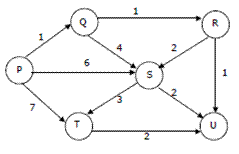
\includegraphics[width=7cm]{shortest.png}
  \end{center}
\end{figure}
В каком порядке будут вычисляться кратчайшие расстояния до вершин?
\begin{checkboxes}
\choice {\tt P, Q, R, S, T, U}
\CorrectChoice {\tt P, Q, R, U, S, T}
\choice {\tt P, Q, R, U, T, S}
\choice {\tt P, Q, T, R, U, S}
\end{checkboxes}

\nomorequestions

\end{questions}

\end{document}
